\special{dvipdfmx:config z 0}
\documentclass[12pt, a4paper, oneside]{ctexbook}
\usepackage{amsmath, amsthm, amssymb, bm, graphicx, hyperref, mathrsfs, float, subfigure, svg}
\usepackage{listings}
\usepackage{ctex}

% 用来设置附录中代码的样式

\lstset{
    basicstyle          =   \sffamily,          % 基本代码风格
    keywordstyle        =   \bfseries,          % 关键字风格
    commentstyle        =   \rmfamily\itshape,  % 注释的风格,斜体
    stringstyle         =   \ttfamily,  % 字符串风格
    flexiblecolumns,                % 别问为什么,加上这个
    numbers             =   left,   % 行号的位置在左边
    showspaces          =   false,  % 是否显示空格,显示了有点乱,所以不现实了
    numberstyle         =   \zihao{-5}\ttfamily,    % 行号的样式,小五号,tt等宽字体
    showstringspaces    =   false,
    captionpos          =   t,      % 这段代码的名字所呈现的位置,t指的是top上面
    frame               =   lrtb,   % 显示边框
}

\lstdefinestyle{Python}{
    language        =   Python, % 语言选Python
    basicstyle      =   \zihao{-5}\ttfamily,
    numberstyle     =   \zihao{-5}\ttfamily,
    keywordstyle    =   \color{blue},
    keywordstyle    =   [2] \color{teal},
    stringstyle     =   \color{magenta},
    commentstyle    =   \color{red}\ttfamily,
    breaklines      =   true,   % 自动换行,建议不要写太长的行
    columns         =   fixed,  % 如果不加这一句,字间距就不固定,很丑,必须加
    basewidth       =   0.5em,
}

\title{{\Huge{\textbf{Chapter1 神经元和数学方法}}}}
\author{黄志权}
\date{\today}
\linespread{1.5}
\newtheorem{theorem}{定理}[section]
\newtheorem{definition}[theorem]{定义}
\newtheorem{lemma}[theorem]{引理}
\newtheorem{corollary}[theorem]{推论}
\newtheorem{example}[theorem]{例}
\newtheorem{proposition}[theorem]{命题}
\CTEXsetup[format={\Large\bfseries}]{section}

\begin{document}

\maketitle

\pagenumbering{roman}
\setcounter{page}{1}

\newpage
\pagenumbering{Roman}
\setcounter{page}{1}
\tableofcontents
\newpage
\setcounter{page}{1}
\pagenumbering{arabic}

\chapter{LIF模型(Leaky-Integrate-and-fire models)}
神经元的动力模型可以被简化为:树突接收若干的脉冲信号,并积累到细胞膜上,致使细胞膜电压改变,从而产生动作电位。LF模型则是将动作电位描述成事件的模型。

\section{膜电压$u(t)$演变的线性微分方程推导}
对于神经元细胞,我们可以将其想象为如下的RC电路。细胞膜就像是一个与电阻并联的电容器,而电阻连接着一个电压为$u_{rest}$电池。当没有外界输入时,膜电压$u(t)$为初始值$u_{rest}$;当有外界脉冲输入时,相当于给电容提供电流为$I(t)$的充电,从而改变模电压$u(t)$。//PS:这个电阻也被称为漏电阻。由于在没有外界输入时,膜上电荷会逐渐穿过细胞膜泄露出去,让膜电压回归$u_{rest}$,因此引入一个漏电阻来模拟这种现象。

\begin{figure}[H]
    \centering
    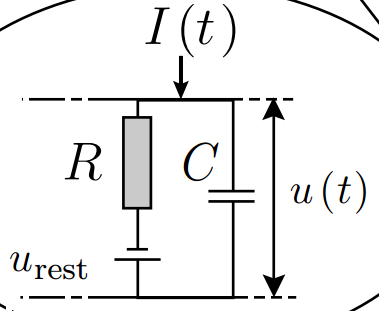
\includegraphics[width=0.3\textwidth]{细胞膜等效电路.png}
    \caption{细胞膜等效电路}
\end{figure} 

考虑$I(t)$不为零的情况,即有外界输入时,来分析膜电压的变化。首先总电流由并联电路支电流和组成$I(t)=I_r+I_C$。即:

\begin{equation}
I(t)=\frac{u(t)-u_{rest}}{R}+C\frac{du(t)}{dt}    
\end{equation}

模仿电路分析,定义膜时间常数(membrane time constant)$\tau _m=RC$。从而可以得到$u(t)$的线性微分方程:

\begin{equation}
    \tau _m\frac{du(t)}{dt}= -[u(t)-u_{rest}] + RI(t)
    \label{微分方程}
\end{equation}

上式在电路分析中称为RC电路响应方程,在神经科学领域称为无源膜方程(equation of a passive membrane)。这个方程的解分为两个部分。即输入脉冲的充电过程(零状态响应),和没有输入脉冲,电压泄露到$u_{rest}$的过程(零状态响应)。首先是输入脉冲的充电过程(零状态响应),我们假设输入电流脉冲在$t_0$时刻是一个幅值为$I_{max}$的方波,则其方程如下:

\begin{equation}
    u(t)=u_{rest}+I_{max}R(1-e^{-\frac{t-t_0}{\tau_m}})
    \label{零状态响应}
\end{equation}

\begin{figure}[H]
    \centering
    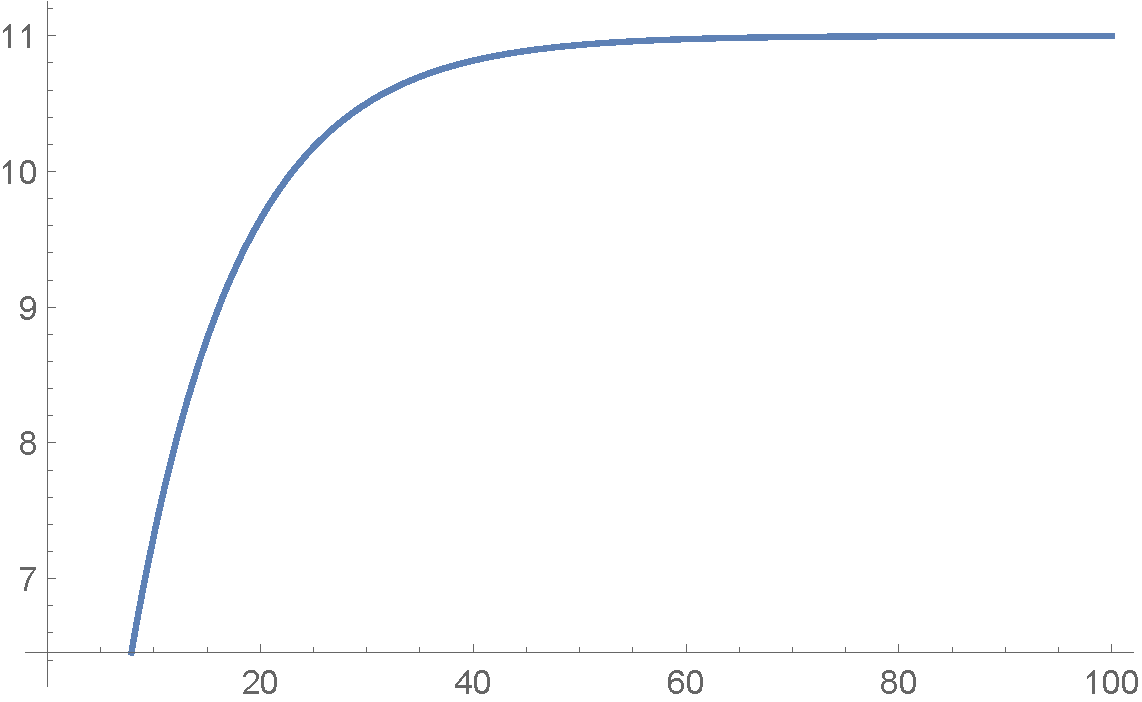
\includegraphics[width=0.5\textwidth]{脉冲充电图.pdf}
    \caption{脉冲充电图}
\end{figure} 

然后是电压泄露到$u_{rest}$的过程(零状态响应),假设脉冲在$t_1$时刻结束:

\begin{equation}
    \begin{aligned}
        u(t)&=u_{rest}+\Delta u Re^{-\frac{t-t_1}{\tau_m}}\\ \Delta u&=u(0)-u_{rest}
    \end{aligned}
    \label{零输入响应}
\end{equation}

\begin{figure}[H]
    \centering
    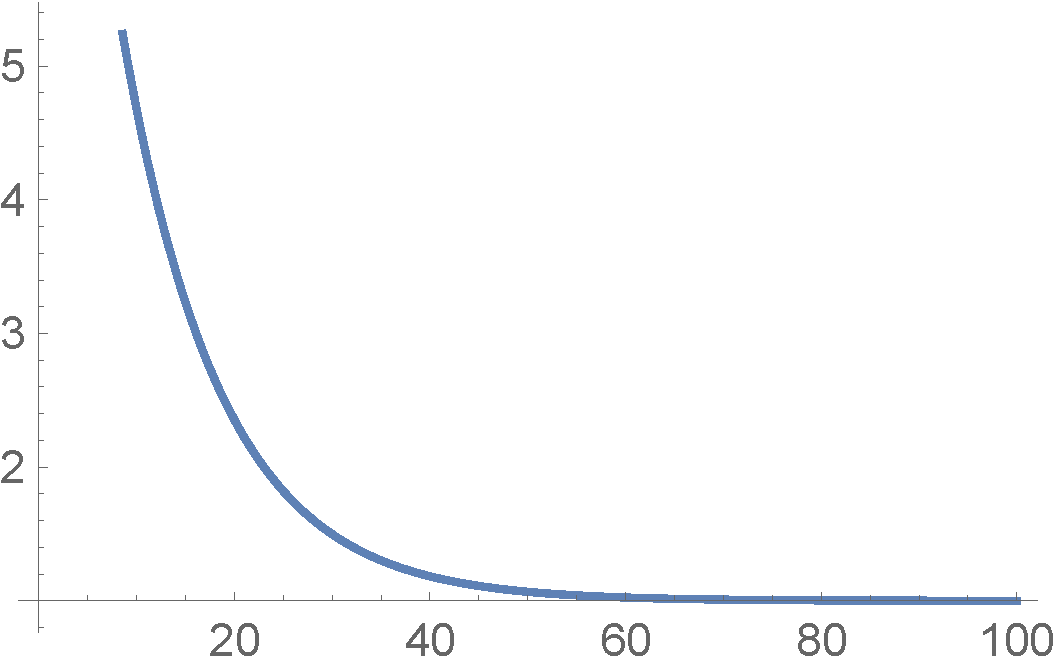
\includegraphics[width=0.5\textwidth]{脉冲放电图.pdf}
    \caption{脉冲放电图}
\end{figure} 

从而,当没有外部脉冲输入的情况下,膜电压会以指数形式衰减到$u_{rest}$。其衰减时间系数$\tau m$一般为10ms,与一般持续1ms的尖峰脉冲相比长了很多。
 
我们可以绘制对于方波输入,膜电压的变化图。我一开始打算利用解析解来绘制,但是发现分段条件太难设置了。因此我选择使用微分方程\ref*{微分方程}来模拟,这样子写成递归函数,会非常简便好看。代码和仿真图如下:\\

\begin{lstlisting}[language=Python]
def U(t_scale, tou, u_t_1, I, R, u_rest):
    return (-(u_t_1 - u_rest) + R*I)/tou*t_scale + u_t_1
\end{lstlisting}

\begin{figure}[H]
    \centering
    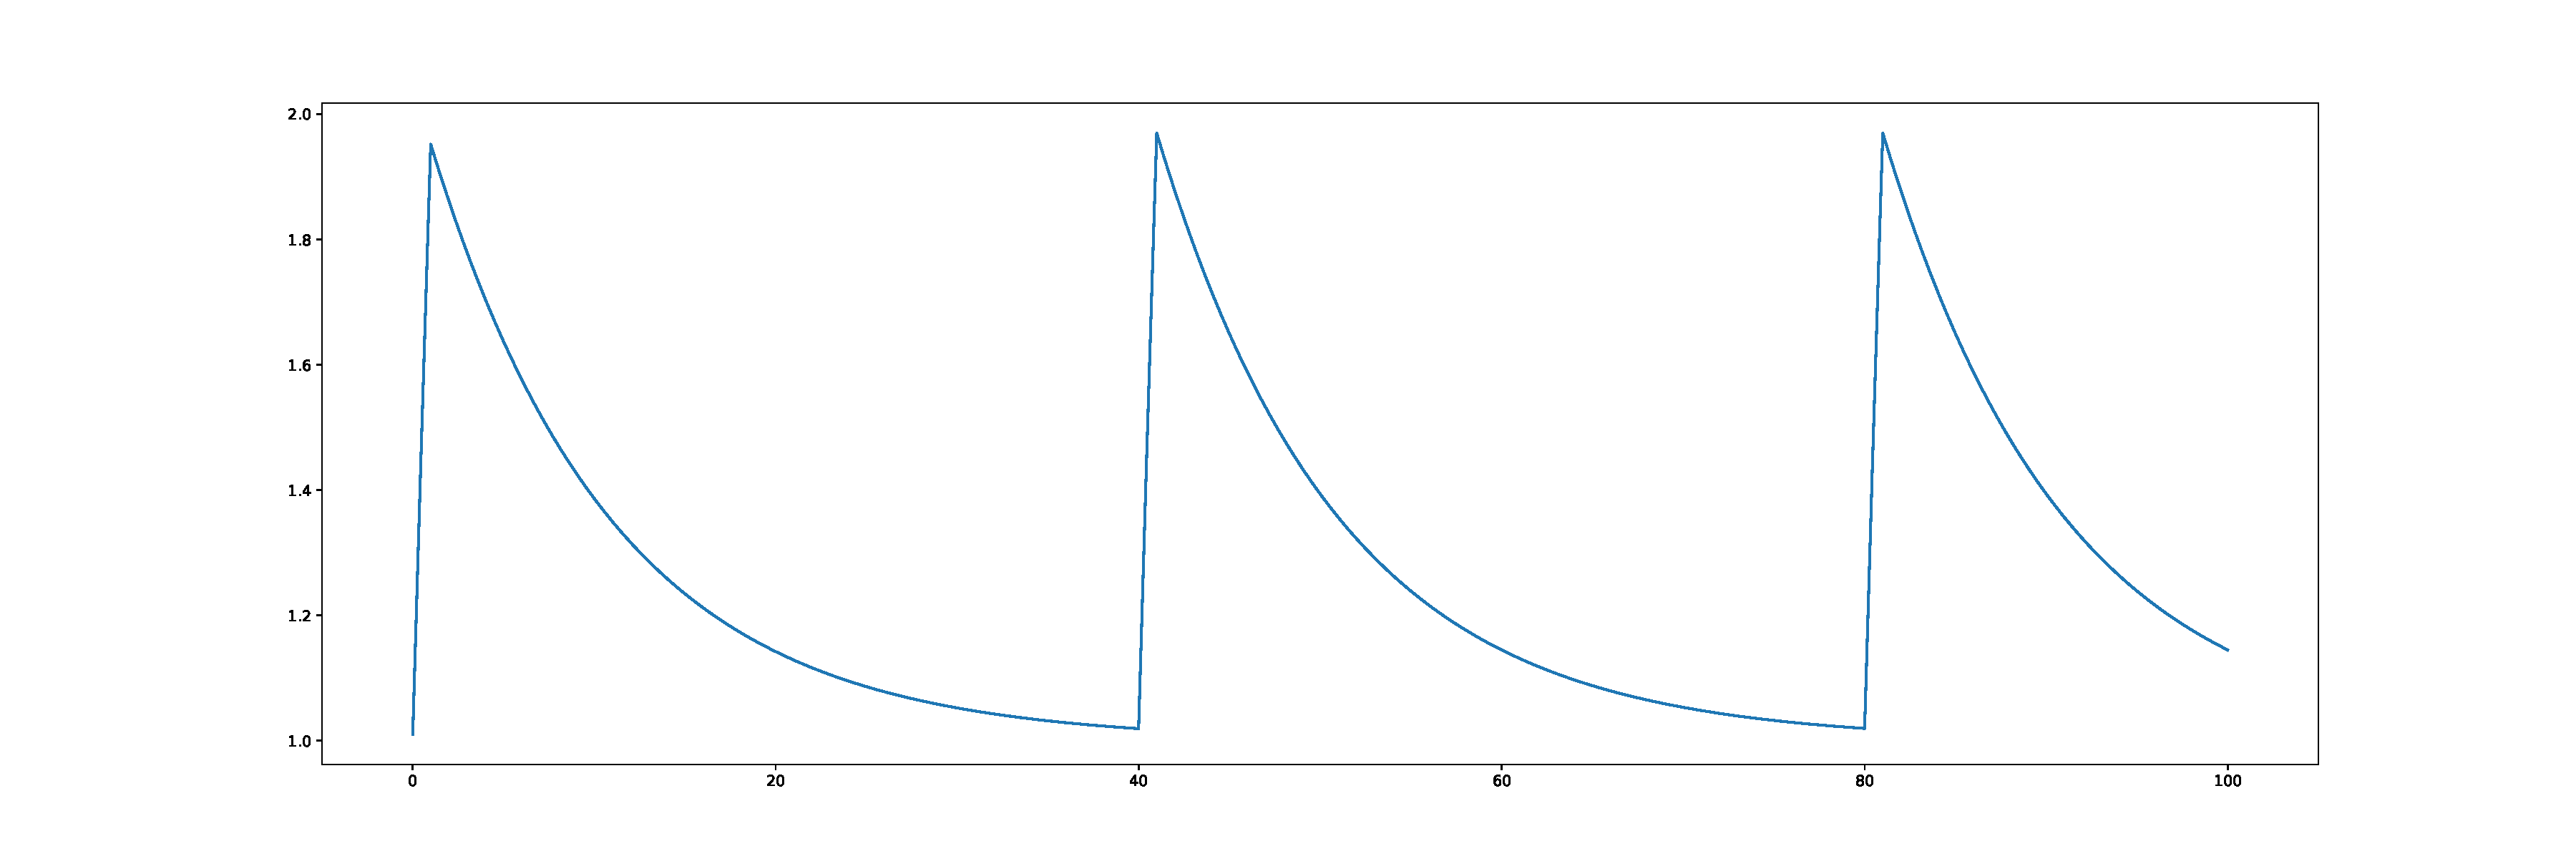
\includegraphics[width=1\textwidth]{方波输入响应图.pdf}
    \caption{方波输入响应图}
\end{figure} 

接下来,考虑输入电流I(t)为一个持续时间为$\Delta$的一个非常短的脉冲。其膜电压轨迹由\ref*{零状态响应}改写得:$u(\Delta)=u_{rest}+I_{max}R(1-e^{-\frac{\Delta}{\tau}})$。对e指数函数做泰勒展开,由于$\Delta$已经很小了,因此只需考虑其一阶情况即可:

\begin{equation}
    u(\Delta)=u_{rest}+I_{max}R\frac{\Delta}{\tau_m}\qquad for \Delta<<\tau_m
    \label{膜电压一阶泰勒}
\end{equation}

然后我们把$\Delta$推至无穷小,并I(t)变形为一个$\delta$函数。从而得到一个总电量$q=I_0\Delta$不变的脉冲。将$q=I_0\Delta$以及$\tau_m=RC$代入上式可得:

\begin{equation}
    u(\Delta)=u_{rest}+\frac{q}{C}
    \label{狄拉克函数}
\end{equation}

然后,可以得到输入脉冲结束后电压泄露到$u_{rest}$的过程。将上式带入\ref*{零输入响应},可得:

\begin{equation}
    u(t)=u_{rest}+\frac{q}{C}e^{-\frac{t-t_0}{\tau_m}}
    \label{脉冲响应}
\end{equation}

从而可以发现,非常窄电流脉冲输入等价于给细胞膜增加了一个$\frac{q}{C}$的电压。当膜电压高于阈值时,会发射一个脉冲,然后膜电压被重置为$u_{r}$,一定要注意,$u_{r}!=u_{rest}$,而是比$u_{rest}$要低一些。记在$t^f$时刻发射了脉冲。那么发射脉冲序列可以用狄拉克求和表示:

\begin{equation}
    S(t)=\sum \delta (t-t^f)
\end{equation}

前面\ref*{零状态响应}和\ref*{零输入响应}零状态响应和零输入响应描述的都是I(t)为恒定状态的情况。下面考虑I(t)为连续的变化信号的情况。由于离散的电流I输入实质上是给细胞膜引入一个$\Delta u=\frac{q}{C}=IR$的电压变化,因此连续变化的I(t)输入即公式\ref*{脉冲响应}与I(t)的卷积:

\begin{equation}
    \begin{aligned}
        u(t)&=u_{rest}+\frac{q}{C}e^{-\frac{t}{\tau_m}}\\
        &=u_{rest}+IRe^{-\frac{t}{\tau_m}}\\
        &=u_{rest}+RI(t)\bigotimes e^{-\frac{t}{\tau_m}}\\
        &=u_{rest}+R\int_0^{+\infty}I(t-s)e^{-\frac{s}{\tau_m}}d\frac{s}{\tau_m}\\
        &=u_{rest}+\frac{R}{\tau_m}\int_0^{+\infty}I(t-s)e^{-\frac{s}{\tau_m}}ds
    \end{aligned}
    \label{卷积}
\end{equation}

上面的式子相当于把输入电流分成无数多小的脉冲,每一个脉冲都会产生$\Delta ue^{-\frac{t}{\tau_m}}$的膜电压变化,然后全部积分起来。那么,同理,我们也可以用同样的方式描述发射脉冲的过程。发射一个脉冲,等价于膜上减少了$\vartheta -u_{r}$的电压,考虑到发射脉冲是离散的,因此我们可以表示为:

\begin{equation}
    \sum_f -(\vartheta -u_{r})e^{-\frac{t-t^f}{\tau_m}}
\end{equation}

因此,描述LF整个输入-输出的膜电压函数为:

\begin{equation}
    u(t)=u_{rest}+\sum_f -(\vartheta -u_{r})e^{-\frac{t-t^f}{\tau_m}}+\frac{R}{\tau_m}\int_0^{+\infty}I(t-s)e^{-\frac{s}{\tau_m}}ds
\end{equation}

\section{输入电流为周期性驱动及其傅里叶变换}

下面我们分析输入电流I(t)为周期性函数时,其膜电压响应的形式。我们定义$\kappa (s)=\frac{1}{C}e^{\frac{s}{\tau_m}}$,则输入电流引起的膜电压的响应可以写作:

\begin{equation}
    u(t)=\int_0^{+\infty}I(t-s)\kappa (s)ds
    \label{卷积公式}
\end{equation}

它具有很漂亮的滤波器的形式,可以看做是滤波器$\kappa(s)$对输入电流I(t)卷积。利用傅里叶变换(Fourier transform)可以得到其频域响应:

\begin{equation}
    u(\omega )=I(\omega )\kappa (\omega )
\end{equation}

现在我们考虑$I(t)=I_0e^{i\omega t}$,代入\ref*{卷积公式}可得:

\begin{equation}
    \begin{aligned}
        u(t)&=\int_0^{+\infty}\kappa (s)e^{-i\omega s}dsI_0e^{i\omega t}\\
        &=\kappa (\omega)I_0e^{i\omega t}
    \end{aligned}
\end{equation}

考虑$u(t)=u_0e^{i(\phi \kappa(\omega)+\omega t)}$,那么其实部增益就可以写作:

\begin{equation}
    \frac{u_0}{I_0}=|\kappa (\omega)|=\int_0^{+\infty}\kappa (s)e^{-i\omega s}ds=\frac{1}{C}|\frac{\tau_m}{1+i\omega \tau_m}|
\end{equation}

由于$\omega \tau_m\gg 1$,因此增益约等于$\frac{1}{C\omega}$。因此,其电压增益和输入频率成反比。下面我在python中试验一下嘿嘿。利用Brian2开源包构建LIF模型,频率从50Hz-500Hz,我们观察其spike的次数。可以看到,spike次数随频率增加有减少的趋势,一定程度上验证了上面的增益公式。

\begin{figure}[H]
    \centering
    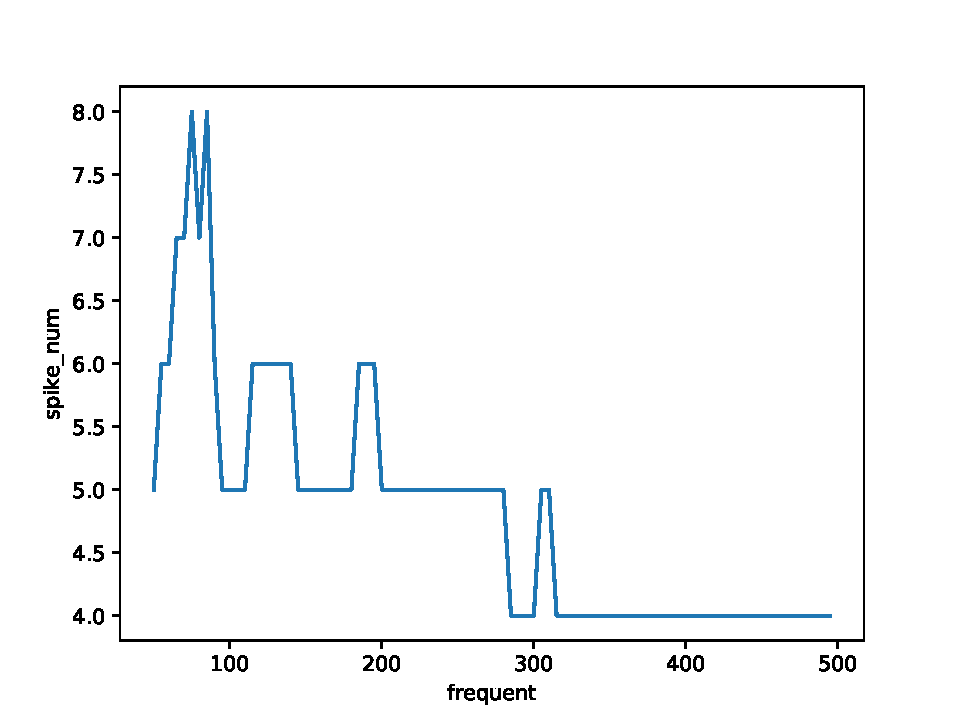
\includegraphics[width=0.5\textwidth]{增益和频率的关系.pdf}
    \caption{增益和频率的关系图}
\end{figure} 

\section{LIF模型的局限性}

我们介绍几种生物学上常见的神经元并以此阐述LIF模型的局限性。如下图所示:

\begin{figure}[H]
    \centering
    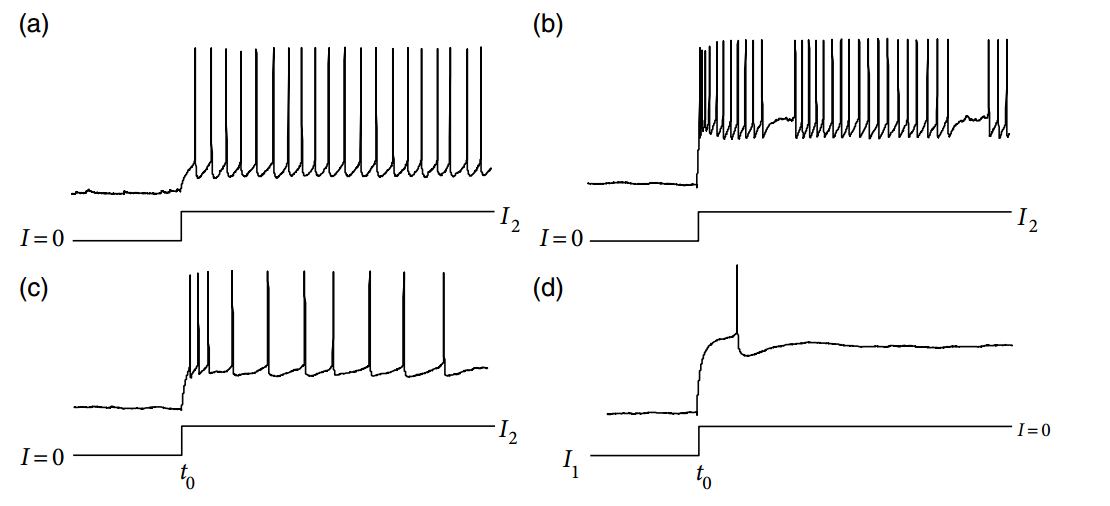
\includegraphics[width=1\textwidth]{四种神经元.png}
    \caption{四种神经元}
\end{figure}

图(a)所示就是LIF模型的神经元,对于一个持续的电流输入,由于神经元在每一次spike时都会重置为$u_{r}$,因此输出的spike序列是一个周期性的序列,这一类神经元也被称为\textbf{快速神经元(fast-spike neurons)}。图(b)所示的神经元叫做\textbf{突发口吃神经元(bursting and stuttering neurons)},它的特点是对于一个持续的电流输入,在一段时间内表现出周期性的输出,又非周期的出现一段长时间的不应期。图(c)所示的神经元叫做\textbf{适应性神经元(adaptation neurons)},与快速神经元不同,它具有适应性,它会积累输入的变化,在一段时间后变成稳定的脉冲输出。最后一种是\textbf{抑制后反弹神经元( post-inhibitory rebound neurons)},它会在输入停止后出现一个尖峰脉冲。上述的神经元在后面的章节中会做进一步讨论。

\section{总结}
由此,我们得到了神经元膜电压的积分方程,以及脉冲发射的方程。

\begin{equation}
    \begin{aligned}
        \tau _m\frac{du(t)}{dt}= -[u(t)-u_{rest}] + RI(t)\\
        \text{If}\quad u(t)=\vartheta \quad then \lim_{\delta \to 0;\delta>0} u(t+\delta)=u_r 
    \end{aligned}
\end{equation}

这个方程很简洁,也很好。但是在实际的神经元实验中,神经元会出现不应期(refractory)和适应性(adaptation)。不应期好处理。适应性考虑如下办法:每输出一个脉冲,给阈值$\vartheta$加一个小量,当输出脉冲为零(即静止状态时),阈值$\vartheta$衰减为初始值。仿照电路响应的微分方程,可以得到如下形式:公式中$\tau_{\text{adapt}}$为适应的时间常数,根据神经科学的实验,一般为几百毫秒。

\begin{equation}
    \tau_{\text{adapt}}\frac{\mathbf{d}}{\mathbf{d}t}\vartheta(t)=-[\vartheta(t)-\vartheta_0]+\theta\sum\limits_f\delta(t-t^f)
\end{equation}

\section{练习题}

\textbf{1、考虑突触输入电流为$\frac{q}{\tau_s}e^{-\frac{t-t_f}{\tau_s}}$($t>t_f$),$t_f$是电流到达突触的时间。}\\
\textbf{(a)求膜电压响应}\\\\
代入公式\ref*{卷积},求解其卷积响应即可。我的信号与系统有点忘光了,求了蛮久,响应如下(没化简):

\begin{equation}
    u(t)=u_{reset}+\frac{qR}{\tau_m-\tau_s}e^{-\frac{t-t_f}{\tau_s}}[e^{(t-t_f)(\frac{1}{\tau_s}-\frac{1}{\tau_m})}-1]
    \label{1.a的解}
\end{equation}

在mathematica文件\href{./exercise/exercise.nb}{exercise.nb}中验证了上式的正确性。并绘制了响应图

\begin{figure}[H]
    \centering
    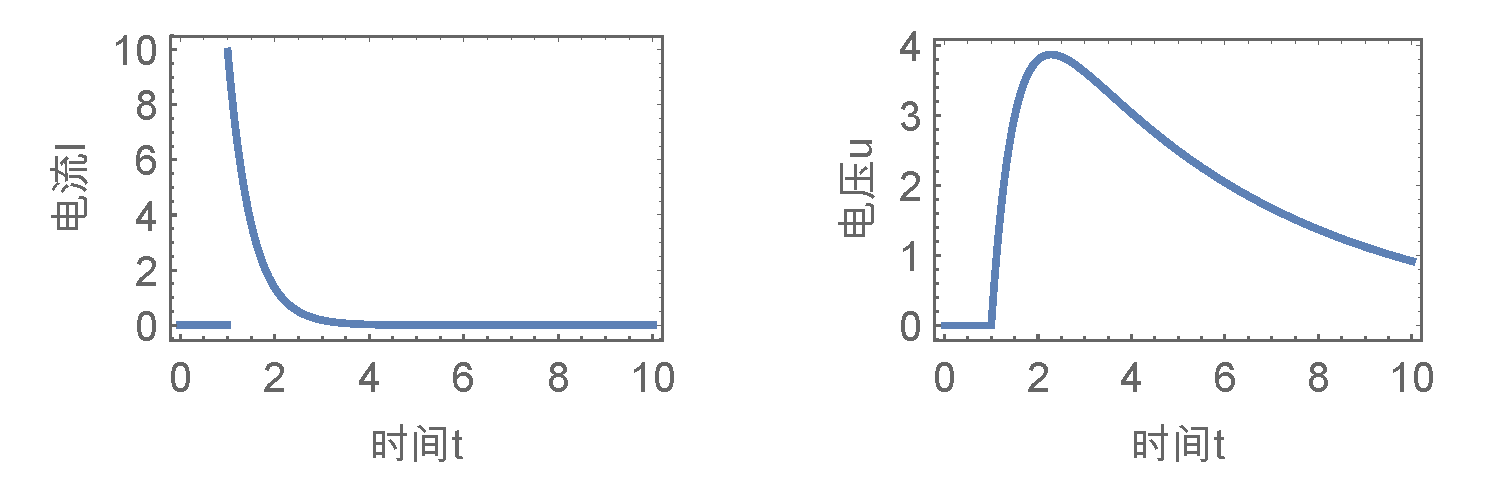
\includegraphics[width=1\textwidth]{exercise/1.a.pdf}
    \caption{1.apdf}
\end{figure}

\textbf{(b)在(a)的解中,取极限$\tau_s\to\tau_m$,并证明响应与$[t-t^{f}]\exp[-\frac{t-t^{f}}{\tau_\text{s}}]$成正比。这种形式的函数有时候被称为$\alpha$函数。}\\\\

显然,我们先计算如下部分:

\begin{equation}
    \begin{aligned}
        &\lim_{\tau_s\to\tau_m}=\frac{e^{(t-t_f)(\frac{1}{\tau_s}-\frac{1}{\tau_m})}-1}{\tau_s-\tau_m}\\
        &\text{利用等价无穷小}\\
        &=\lim_{\tau_s\to\tau_m}=\frac{(t-t_f)(\frac{1}{\tau_s}-\frac{1}{\tau_m})}{\tau_m-\tau_s}\\
        &=\frac{t-t_f}{\tau_m\tau_s}
    \end{aligned}
\end{equation}

代入公式\ref*{1.a的解},可得:

\begin{equation}
    u(t)=u_{reset}+\frac{qR}{\tau_m\tau_s}e^{-\frac{t-t_f}{\tau_s}}[t-t_f]
\end{equation}

从而可以证明,$u(t)$确实是与$[t-t^{f}]\exp[-\frac{t-t^{f}}{\tau_\text{s}}]$成正比的。

\textbf{(c)在(a)的解中,取极限$\tau_s\to0$。看看能不能把你的结论和狄拉克函数联系在一起?}\\\\

对公式\ref*{1.a的解}取极限,得:

\begin{equation}
    \begin{aligned}
        &\lim_{\tau_s\to0}u_{reset}+\frac{qR}{\tau_m-\tau_s}e^{-\frac{t-t_f}{\tau_s}}[e^{(t-t_f)(\frac{1}{\tau_s}-\frac{1}{\tau_m})}-1]\\
        &=\lim_{\tau_s\to0}u_{reset}+\frac{qR}{\tau_m-\tau_s}[e^{-\frac{t-t_f}{\tau_m}}-e^{-\frac{t-t_f}{\tau_s}}]\\
        &=u_{reset}+\frac{qR}{\tau_m}e^{-\frac{t-t_f}{\tau_m}}\qquad(t>t_f)
    \end{aligned}
\end{equation}

可以看到,当$\tau_s\to0$时,膜电压变化公式退化为公式\ref*{脉冲响应},即输入为狄拉克脉冲时的情形。同样,我们通过mathematica仿真一下。非常漂亮的一张图。

\begin{figure}[H]
    \centering
    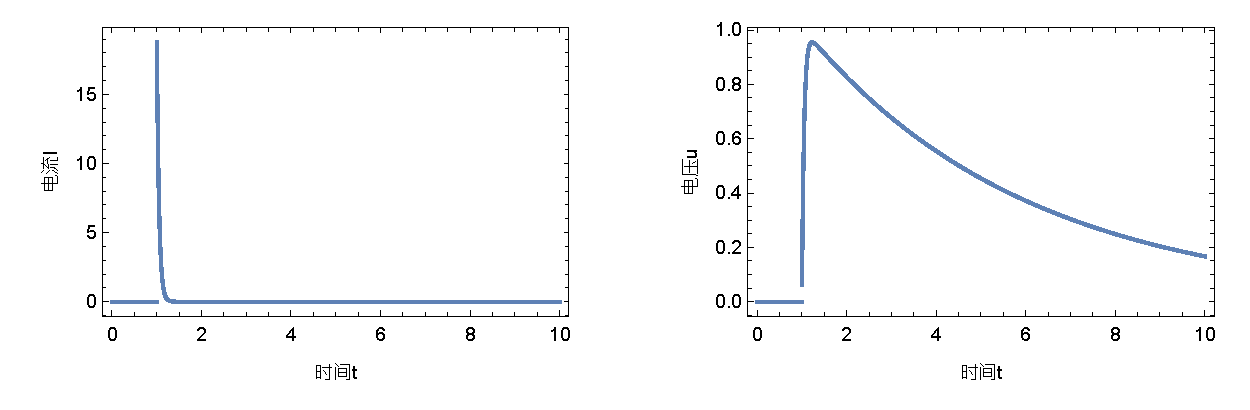
\includegraphics[width=1\textwidth]{exercise/1.c.pdf}
    \caption{1.cpdf}
\end{figure}

\textbf{2、考虑突触输入电流为随时间变化的电流输入(Time-dependent solution)。则可知其膜电压变化的解为公式\ref*{卷积}。现在我们交换公式\ref*{卷积}里卷积的顺序(卷积交换顺序不影响结果)。然后对该式求微分,比较一下微分方程两端的结果。}\\

这一段推导到了一上午。主要是高数的很多知识都忘记了。

\begin{equation}
    \begin{aligned}
        u(t)&=u_{rest}+\frac{R}{\tau_m}\int_0^\infty e^{-\frac{t-s}{\tau_m}}I(s)ds\\
        &\text{两边求导}\\
        \frac{du(t)}{dt}&=\frac{1}{dt}[u_{rest}+\frac{R}{\tau_m}\int_0^\infty e^{-\frac{t-s}{\tau_m}}I(s)ds]\\
    \end{aligned}
\end{equation}

这个地方踩了一个大坑,实际的积分上限是t,($t\to\infty$)区间没有意义,如果上限使用$\infty$,计算不出结果。

\begin{equation}
    \begin{aligned}
        \frac{du(t)}{dt}&=\frac{1}{dt}[u_{rest}+\frac{R}{\tau_m}\int_0^t e^{-\frac{t-s}{\tau_m}}I(s)ds]\\
        \frac{du(t)}{dt}&=\frac{1}{dt}[u_{rest}+\frac{R}{\tau_m}e^{-\frac{t}{\tau_m}}\int_0^t e^{\frac{s}{\tau_m}}I(s)ds]\\
    \end{aligned}
\end{equation}

这里链式积分和不定积分求导,应用$\Phi'(x)=\frac{d}{dx}\int_{\phi(x)}^{\varphi(x)}f(t)dt=f[\varphi(x)]\varphi'(x)-f[\phi(x)]\phi'(x)$

\begin{equation}
    \begin{aligned}
        \frac{du(t)}{dt}&=\frac{R}{\tau_m}\frac{-1}{\tau_m}[\int_0^t e^{-\frac{t-s}{\tau_m}}I(s)ds+\frac{R}{\tau_m}I(t)]\\
        \tau_m\frac{du(t)}{dt}&=-[u(t)-u_{rest}]+RI(t)\\
    \end{aligned}
\end{equation}

最终得到的形式和公式\ref*{微分方程}一致。这也正常,毕竟本身就是公式\ref*{微分方程}的一个解。

\textbf{3、假设在$t_f$时刻神经递质被传递到突触出,浓度为$\tau_x\frac{\text{d}x}{\text{d}t}=-x+\delta(t-t_f)$,神经递质与突触受体结合,打开离子通道,产生电流为$\tau_s\frac{\text{d}I}{\text{d}t}=-I+I_0x(t)$,并引起膜电压变化为$\tau_m\frac{\text{d}u}{\text{d}t}=-u+RI(t)$,求出膜电压变化公式。这三个传递构成了一个线性方程组(Chain of linear equations)}

对三条线性方程依次求解即可,我决定利用mathematica来求解,解得:

\begin{equation}
    x(t)=\frac{1}{\tau_x}e^{-\frac{t-t_f}{\tau_x}}\theta(t-t_f)
\end{equation}

\begin{equation}
    I(t)=\frac{I_0(e^{\frac{t_f-t}{\tau_s}}-e^{\frac{t_f-t}{\tau_x}})}{\tau_s-\tau_x}\theta (t-t_f)
\end{equation}

\begin{equation}
    \begin{aligned}
        u(t)&=I_0 R \theta (t-t_f) e^{-\frac{t}{\tau_m}-\frac{t}{\tau_s}-\frac{t}{\tau_x}}\\
        &(\tau_s (\tau_x-\tau_m) e^{\frac{t}{\tau_m}+\frac{t}{\tau_x}+\frac{t_f}{\tau_s}}+\\
        &\tau_m (\tau_s-\tau_x) e^{\frac{t}{\tau_s}+\frac{t}{\tau_x}+\frac{t_f}{\tau_m}}+\\
        &\tau_x (\tau_m-\tau_s) e^{\frac{t}{\tau_m}+\frac{t}{\tau_s}+\frac{t_f}{\tau_x}})\\
        &/((\tau_s-\tau_m) (\tau_m-\tau_x) (\tau_s-\tau_x))
    \end{aligned}
\end{equation}

具有某种规律性的美感。本章完结!

\chapter{离子通道和 Hodgkin–Huxley 模型}

Hodgkin–Huxley模型其等效电路图和LIF模型的区别是它考虑的钠离子和钾离子两个通道,并且给出了生物学上的具体意义。电路图如下所示:

\begin{figure}[H]
    \centering
    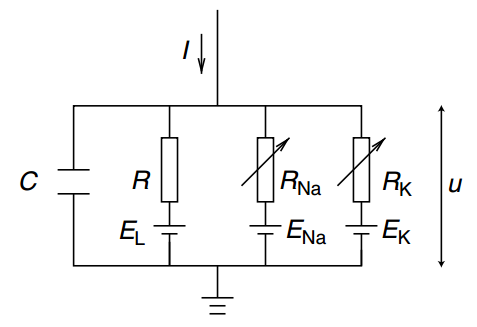
\includegraphics[width=0.7\textwidth]{HH模型电路图.png}
    \caption{HH模型电路图}
\end{figure}

它一共有3个支路,$R_{Na}、R_{K}$支路是钠离子、钾离子通道的等效电阻,$E_{Na}、E_{K}$是钠离子、钾离子的通道电势。这个电势是由离子浓度差引起的。它有一个专业名词叫能斯特电势(Nernst potential)。



\end{document}